\documentclass[11pt]{article}

\usepackage[margin=1in]{geometry}
\usepackage[T1]{fontenc}
\usepackage[utf8]{inputenc}
\usepackage{lmodern}
\usepackage{microtype}
\usepackage{amsmath, amssymb, amsthm, bm}
\usepackage{booktabs}
\usepackage{multirow}
\usepackage{graphicx}
\usepackage{float}
\usepackage{enumitem}
\usepackage{hyperref}
\usepackage[nameinlink,capitalise,noabbrev]{cleveref}
\usepackage{authblk}
\usepackage{setspace}
\usepackage{xcolor}

\graphicspath{{../figures-progress/}}

\hypersetup{
  colorlinks=true,
  linkcolor=blue,
  citecolor=blue,
  urlcolor=blue
}

%% ----------------------------------------------------------------
%%  DRAFT STATUS MARKERS
%%  \status{text} — inline marker for incomplete items
%%  \pending{text} — marks a section that needs data from a pending experiment
%% ----------------------------------------------------------------
\newcommand{\status}[1]{\textcolor{red}{\textbf{[#1]}}}
\newcommand{\pending}[1]{\textcolor{orange}{\textbf{[PENDING: #1]}}}

\title{Do Simple Physics Priors Change Empirical Scaling in Scientific Machine Learning?\\
\large A Controlled Lotka--Volterra Case Study}

\author[1]{Lucas Perrier}
\affil[1]{Affiliation placeholder}
\date{Draft --- \today}

\begin{document}

\maketitle

%% ================================================================
%%  ABSTRACT
%% ================================================================
\begin{abstract}
Physics-informed learning methods are typically evaluated at fixed model and dataset sizes, making it difficult to determine whether a physical prior changes learning behavior systematically or merely shifts performance in isolated settings.
We propose empirical scaling laws as a diagnostic framework for physics priors and demonstrate the approach on fixed-horizon flow-map prediction for the Lotka--Volterra system.
We compare a plain multilayer perceptron against three physics-regularized variants---a single-step ODE-residual prior (midpoint rule), a composite two-step ODE-residual prior (reduced-bias midpoint), and a conservation-law prior---across five model capacities and eight dataset sizes, fitting
\[
E(N,D) \approx E_\infty + aN^{-\alpha} + bD^{-\beta}.
\]
The three priors produce three qualitatively distinct scaling signatures, forming a diagnostic taxonomy.
The \emph{single-step midpoint} prior, which incurs $\sim\!15\%$ irreducible approximation error at the tested horizon, raises the error floor to $\hat{E}_\infty \approx 0.011$ and compresses both scaling exponents ($\hat{\alpha} \approx 0.18$, $\hat{\beta} \approx 0.54$), making the model insensitive to additional data or capacity.
The \emph{composite midpoint} prior, whose two-step discretization reduces the ground-truth residual by $\sim\!24\times$, recovers healthy scaling with steeper exponents ($\hat{\alpha} \approx 2.0$, $\hat{\beta} \approx 1.0$) than the plain baseline ($\hat{\alpha} \approx 0.93$, $\hat{\beta} \approx 0.87$) and a near-zero floor ($\hat{E}_\infty \approx 0.001$).
The \emph{conservation-law} prior, which is exact but informationally weak (constraining a single scalar on a vector-valued output), introduces bimodal optimization failures that worsen with model capacity.
These contrasting outcomes demonstrate that scaling-law analysis distinguishes not only whether a prior helps, but \emph{how} it modifies the learning surface: biased priors raise the error floor, reduced-bias priors steepen scaling exponents, and exact-but-weak priors corrupt the surface stochastically.
\end{abstract}

%% ================================================================
%%  INTRODUCTION
%% ================================================================
\section{Introduction}

Scientific machine learning (SciML) aims to combine data-driven models with scientific structure such as governing equations, invariants, symmetries, and conservation laws~\cite{willard2022,karpatne2022}.
A central hope is that such structure improves data efficiency, robustness, and interpretability.
However, comparisons between physics-informed and purely data-driven methods are often made at only a few fixed dataset sizes and model capacities.
As a result, it remains unclear whether physics-informed priors change learning in a systematic way or simply shift performance in isolated experimental settings.

In mainstream machine learning, empirical scaling laws have become a useful lens for understanding how test error changes as a function of model size, dataset size, and compute~\cite{kaplan2020,hestness2017}.
By contrast, comparable scaling-based evaluation is still underdeveloped in SciML.
This is a notable gap because scientific learning problems are especially sensitive to regime: task difficulty depends not only on sample count, but also on time horizon, parameter variability, discretization, optimization stability, and the form of the physical prior itself.

This paper studies a controlled instance of that broader question.
We consider fixed-horizon flow-map prediction on the Lotka--Volterra system and ask:

\begin{quote}
Do different physics priors produce distinguishable scaling signatures, and can these signatures diagnose the quality of the prior?
\end{quote}

We study \emph{three} physics priors on the same system and task: a single-step ODE residual (biased), a composite two-step ODE residual (reduced-bias), and an exact conservation-law invariant.
This triad is chosen to span a range of prior accuracy and informational content, enabling a taxonomy of prior--scaling interactions.

Our contributions are:

\begin{enumerate}[leftmargin=*, itemsep=0.3em]
    \item A scaling-law diagnostic protocol for evaluating physics priors on controlled dynamical systems, combining scaling fits with $\lambda$-sensitivity analysis and ground-truth residual checks.
    \item A two-axis scaling study over model capacity ($N$) and dataset size ($D$) for four models---a plain baseline plus three physics-regularized variants---totalling over 1{,}400 training runs.
    \item A three-way taxonomy of prior--scaling interactions: a \emph{biased} prior raises the error floor and compresses exponents; a \emph{reduced-bias} prior recovers and steepens scaling; an \emph{exact-but-weak} prior corrupts the scaling surface through stochastic optimization failure.
    \item Empirical evidence that scaling exponents and error floors are \emph{more informative} than point-wise comparisons: two priors that both underperform the baseline in absolute terms produce fundamentally different scaling signatures with distinct implications for the practitioner.
\end{enumerate}

%% ================================================================
%%  RELATED WORK
%% ================================================================
\section{Related Work}

\subsection{Physics-informed scientific machine learning}

Physics-informed learning methods inject scientific structure into machine learning models in several ways.
Soft approaches typically introduce residual penalties derived from governing equations~\cite{raissi2019pinn,cuomo2022}, with variants such as fractional PINNs~\cite{pang2019fpinns}.
Harder approaches build physical structure directly into the architecture or parameterization~\cite{willard2022,chen2018node}.
Operator-learning architectures such as DeepONet~\cite{lu2019deeponet} and Fourier Neural Operators~\cite{li2020fno} learn solution operators between function spaces.
These methods have been applied to fluid dynamics, climate modelling~\cite{kashinath2021}, and multiscale closure problems~\cite{sanderse2024}.
However, most evaluations are architecture- and problem-specific, comparing models at fixed dataset sizes and capacities~\cite{cuomo2022,ren2025}.
Physics-informed architectures also exhibit non-trivial optimization pathologies: PINNs can fail to train due to ill-conditioned neural tangent kernels~\cite{wang2022ntk}.

\subsection{Empirical scaling laws}

Empirical scaling laws describe how performance changes as a function of data, model size, or compute.
In natural language processing and vision, such laws have proven useful both descriptively and operationally~\cite{kaplan2020,hestness2017,henighan2020}.
They provide a compact summary of learning efficiency and can reveal regime changes or diminishing returns.
Recent work explains scaling phenomena through variance-limited and resolution-limited regimes~\cite{bahri2024}, while constructive models can predict generalization error across scales~\cite{rosenfeld2019}.
A recent survey documents similar power-law behavior across a wide range of machine learning settings~\cite{wang2024scaling}.

\subsection{Scaling as an evaluation lens for SciML}

The use of scaling laws in SciML is still limited.
Theoretical work on neural scaling for elliptic PDEs has begun to establish generalization bounds~\cite{lu2021elliptic}, but these results are confined to specific PDE classes.
There remains a need for controlled empirical work asking whether physical priors change the shape of learning curves in a reproducible and interpretable way.

%% ================================================================
%%  PROBLEM SETTING
%% ================================================================
\section{Problem Setting}

\subsection{Task formulation}

We study supervised fixed-horizon flow-map prediction for the Lotka--Volterra system.
Let $\bm{x}(t) = (u(t), v(t)) \in \mathbb{R}^2$ denote the system state.
Given an initial condition $\bm{x}_0$ and a fixed prediction horizon $T > 0$, the learning task is to approximate the flow map
\[
\Phi_T : \bm{x}_0 \mapsto \bm{x}(T).
\]
This formulation provides a well-defined supervised target while avoiding the confounding effects of long autoregressive rollout.

\subsection{Lotka--Volterra dynamics}

The Lotka--Volterra system is defined by
\begin{align}
\frac{du}{dt} &= \alpha u - \beta uv, \label{eq:lv-prey}\\
\frac{dv}{dt} &= \delta uv - \gamma v, \label{eq:lv-pred}
\end{align}
where $u$ and $v$ denote prey and predator populations, and $\alpha,\beta,\gamma,\delta > 0$ are system parameters.
We use fixed parameters $(\alpha,\beta,\delta,\gamma) = (1.5, 1.0, 1.0, 3.0)$ throughout.

The system possesses an exact first integral (conservation law):
\begin{equation}
H(u,v) = \delta u - \gamma \ln u + \beta v - \alpha \ln v,
\label{eq:lv-invariant}
\end{equation}
satisfying $H(\bm{x}(t)) = H(\bm{x}_0)$ for all $t$.
This invariant plays a central role in our experimental design: it provides an \emph{exact} physics prior that can be contrasted with an \emph{approximate} one.

\subsection{Data generation}

Initial conditions are sampled uniformly from $[0.5, 2.5]^2$.
Ground-truth flow maps are computed using the DOP853 solver (Dormand--Prince 8(5,3)) at tolerances $\texttt{rtol} = 10^{-9}$, $\texttt{atol} = 10^{-11}$, with prediction horizon $T = 1.0$.
The dataset comprises 20{,}000 training pairs, 2{,}000 validation, and 2{,}000 test pairs.
Training subsets of sizes $D \in \{64, 128, 256, 512, 1024, 2048, 4096, 8192\}$ are drawn as nested prefixes of the same shuffled training pool, ensuring that each smaller set is a subset of every larger one.
Three independent data seeds (11, 22, 33) provide distinct pools.

%% ================================================================
%%  MODELS
%% ================================================================
\section{Models}

\subsection{Plain MLP baseline}

Our baseline is a standard multilayer perceptron (MLP) with ReLU activations:
\[
\hat{\bm{x}}_T = f_\phi(\bm{x}_0),
\]
trained to minimize the mean squared error
\[
\mathcal{L}_{\mathrm{data}} = \frac{1}{B}\sum_{i=1}^{B} \left\| f_\phi(\bm{x}_0^{(i)}) - \bm{x}_T^{(i)} \right\|_2^2.
\]
Input and output are standardized using training-set statistics; the loss is computed in normalized space.

\subsection{Capacity grid}

Model capacity $N$ (parameter count) is varied through a fixed architecture grid:

\begin{center}
\begin{tabular}{lcr}
\toprule
Name & Hidden widths & Parameters ($N$) \\
\midrule
Tiny   & $[32, 32]$        & 1{,}218 \\
Small  & $[64, 64]$        & 4{,}482 \\
Medium & $[128, 128]$      & 17{,}154 \\
Large  & $[256, 256]$      & 67{,}074 \\
XLarge & $[256, 256, 256]$ & 132{,}866 \\
\bottomrule
\end{tabular}
\end{center}

\subsection{ODE-residual prior (midpoint)}
\label{sec:midpoint-prior}

The first physics-regularized model augments the data loss with a midpoint-rule ODE residual:
\[
\mathcal{L}_{\mathrm{total}} = \mathcal{L}_{\mathrm{data}} + \lambda_{\mathrm{phys}} \mathcal{L}_{\mathrm{mid}},
\]
where
\[
\mathcal{L}_{\mathrm{mid}} = \frac{1}{B}\sum_{i=1}^{B} \left\| \hat{\bm{x}}_T^{(i)} - \bm{x}_0^{(i)} - T \cdot F\!\left(\tfrac{\bm{x}_0^{(i)} + \hat{\bm{x}}_T^{(i)}}{2}\right) \right\|_2^2
\]
and $F$ is the Lotka--Volterra vector field from \cref{eq:lv-prey,eq:lv-pred}.
This is a first-order implicit-midpoint quadrature approximation to the integral form of the ODE, computed on denormalized (physical) state variables.

\subsection{Conservation-law prior}
\label{sec:conservation-prior}

The second physics-regularized model penalizes violation of the exact first integral:
\[
\mathcal{L}_{\mathrm{total}} = \mathcal{L}_{\mathrm{data}} + \lambda_{\mathrm{phys}} \mathcal{L}_{\mathrm{cons}},
\]
where
\[
\mathcal{L}_{\mathrm{cons}} = \frac{1}{B}\sum_{i=1}^{B} \left( H(\hat{\bm{x}}_T^{(i)}) - H(\bm{x}_0^{(i)}) \right)^2
\]
and $H$ is the invariant from \cref{eq:lv-invariant}.
Unlike the midpoint residual, this prior has zero irreducible error: $\mathcal{L}_{\mathrm{cons}} = 0$ on exact flow-map targets.

\subsection{Composite two-step midpoint prior}
\label{sec:composite-prior}

The third physics-regularized model uses a composite midpoint rule with two half-steps, reducing the discretization bias of the single-step midpoint.
The model outputs a 4-dimensional vector $(\hat{\bm{x}}_{T/2}, \hat{\bm{x}}_T) \in \mathbb{R}^4$, predicting both the midpoint state and the final state.
Only $\hat{\bm{x}}_T$ contributes to the data loss; $\hat{\bm{x}}_{T/2}$ is shaped entirely by the physics loss:
\[
\mathcal{L}_{\mathrm{total}} = \mathcal{L}_{\mathrm{data}}(\hat{\bm{x}}_T, \bm{x}_T) + \lambda_{\mathrm{phys}} \mathcal{L}_{\mathrm{comp}},
\]
where the composite residual applies the midpoint rule on each half-interval:
\begin{align}
\bm{r}_a &= \hat{\bm{x}}_{T/2} - \bm{x}_0 - \tfrac{T}{2}\, F\!\left(\tfrac{\bm{x}_0 + \hat{\bm{x}}_{T/2}}{2}\right), \label{eq:comp-ra} \\
\bm{r}_b &= \hat{\bm{x}}_T - \hat{\bm{x}}_{T/2} - \tfrac{T}{2}\, F\!\left(\tfrac{\hat{\bm{x}}_{T/2} + \hat{\bm{x}}_T}{2}\right), \label{eq:comp-rb} \\
\mathcal{L}_{\mathrm{comp}} &= \frac{1}{B}\sum_{i=1}^{B} \left(\|\bm{r}_a^{(i)}\|^2 + \|\bm{r}_b^{(i)}\|^2\right). \notag
\end{align}
Because the midpoint rule has local truncation error $O(h^3)$ where $h$ is the step size, halving the step from $T$ to $T/2$ reduces the residual on ground-truth targets by approximately $2^2 = 4\times$ per step, and the two-step composite achieves $\sim\!24\times$ lower physics loss on ground truth compared to single-step midpoint ($\mathcal{L}_{\mathrm{comp}}^* \approx 0.006$ vs.\ $\mathcal{L}_{\mathrm{mid}}^* \approx 0.151$).
This design tests whether reducing---but not eliminating---the discretization bias recovers healthy scaling behavior.

%% ================================================================
%%  EXPERIMENTAL DESIGN
%% ================================================================
\section{Experimental Design}

\subsection{Scaling axes}

We vary two quantities systematically:
\begin{itemize}[leftmargin=*]
    \item \textbf{Model capacity} $N$: five sizes from 1{,}218 to 132{,}866 parameters.
    \item \textbf{Dataset size} $D$: eight sizes from 64 to 8{,}192 training samples.
\end{itemize}
The use of nested subsets reduces confounding due to sample composition.

\subsection{Evaluation metric}

The primary metric is the mean relative $\ell_2$ prediction error on the held-out test set, computed in physical (denormalized) coordinates:
\[
E(N,D) = \frac{1}{M}\sum_{i=1}^{M}
\frac{\left\| \hat{\bm{x}}_T^{(i)} - \bm{x}_T^{(i)} \right\|_2}
{\left\| \bm{x}_T^{(i)} \right\|_2 + \varepsilon},
\]
where $\varepsilon > 0$ is a small stability constant.

\subsection{Scaling-law ansatz}

We fit empirical relationships of the form
\begin{equation}
E(N,D) \approx E_\infty + aN^{-\alpha} + bD^{-\beta},
\label{eq:scaling}
\end{equation}
where $E_\infty$ is an asymptotic error floor, $\alpha$ is the capacity-scaling exponent, $\beta$ is the data-scaling exponent, and $a,b > 0$ are fitted coefficients.
The purpose is descriptive and comparative, not predictive.

\subsection{Statistical protocol}

Each $(N, D)$ configuration is run across 3 data seeds $\times$ 3 training seeds $= 9$ replicates.
We report mean and standard error across replicates.
Scaling-law parameters are estimated with 1{,}000 bootstrap samples to produce 95\% confidence intervals.

\subsection{Training details}

All models use Adam with learning rate $10^{-3}$, weight decay $10^{-6}$, batch size $\min(128, D)$, and train for up to 400 epochs with early stopping (patience 40 on validation relative $\ell_2$).
The composite model has a 4-dimensional output; only the last two components ($\hat{\bm{x}}_T$) are used for the data loss and evaluation metric.
The full grid comprises $5 \times 8 \times 9 = 360$ runs per model, totaling 1{,}080 production runs for the three scaling-law models (plain, midpoint, composite), plus 126 conservation-law $\lambda$-sweep runs and 324 midpoint $\lambda$-sweep runs.

%% ================================================================
%%  RESEARCH QUESTIONS
%% ================================================================
\section{Research Questions}

\begin{enumerate}[leftmargin=*, itemsep=0.3em]
    \item Do physics priors produce distinct, interpretable signatures in the scaling surface $E(N,D)$?
    \item Does reducing the discretization bias of an ODE-residual prior recover healthy scaling?
    \item Does an exact but informationally weak prior (conservation law) improve data efficiency?
    \item Can scaling exponents and error floors diagnose prior quality more informatively than point-wise comparisons?
\end{enumerate}

%% ================================================================
%%  RESULTS
%% ================================================================
\section{Results}

\subsection{Plain MLP baseline: scaling behavior}
\label{sec:results-plain}

The plain MLP exhibits clean power-law scaling across both axes.
Representative test errors (mean $\pm$ stderr over 9 replicates):

\begin{center}
\small
\begin{tabular}{lrrrr}
\toprule
& $D = 64$ & $D = 512$ & $D = 2048$ & $D = 8192$ \\
\midrule
Tiny ($N\!=\!1218$)    & $0.0164 \pm 0.0006$ & $0.0055 \pm 0.0002$ & $0.0026 \pm 0.0001$ & $0.0017 \pm 0.0001$ \\
Small ($N\!=\!4482$)   & $0.0103 \pm 0.0005$ & $0.0030 \pm 0.0001$ & $0.0015 \pm 0.0001$ & $0.0010 \pm 0.0000$ \\
Medium ($N\!=\!17154$) & $0.0070 \pm 0.0007$ & $0.0016 \pm 0.0001$ & $0.0010 \pm 0.0000$ & $0.0008 \pm 0.0001$ \\
Large ($N\!=\!67074$)  & $0.0049 \pm 0.0005$ & $0.0011 \pm 0.0000$ & $0.0009 \pm 0.0000$ & $0.0008 \pm 0.0000$ \\
XLarge ($N\!=\!132866$)& $0.0045 \pm 0.0004$ & $0.0012 \pm 0.0000$ & $0.0009 \pm 0.0000$ & $0.0007 \pm 0.0000$ \\
\bottomrule
\end{tabular}
\end{center}

The combined scaling fit yields:
\[
\hat{E}_\infty \approx 0,\quad \hat{\alpha} \approx 0.93,\quad \hat{\beta} \approx 0.87.
\]
These exponents are stable across bootstrap resamples.
The near-zero error floor indicates that adding more data and capacity continues to yield improvement across the tested range.

\begin{figure}[H]
    \centering
    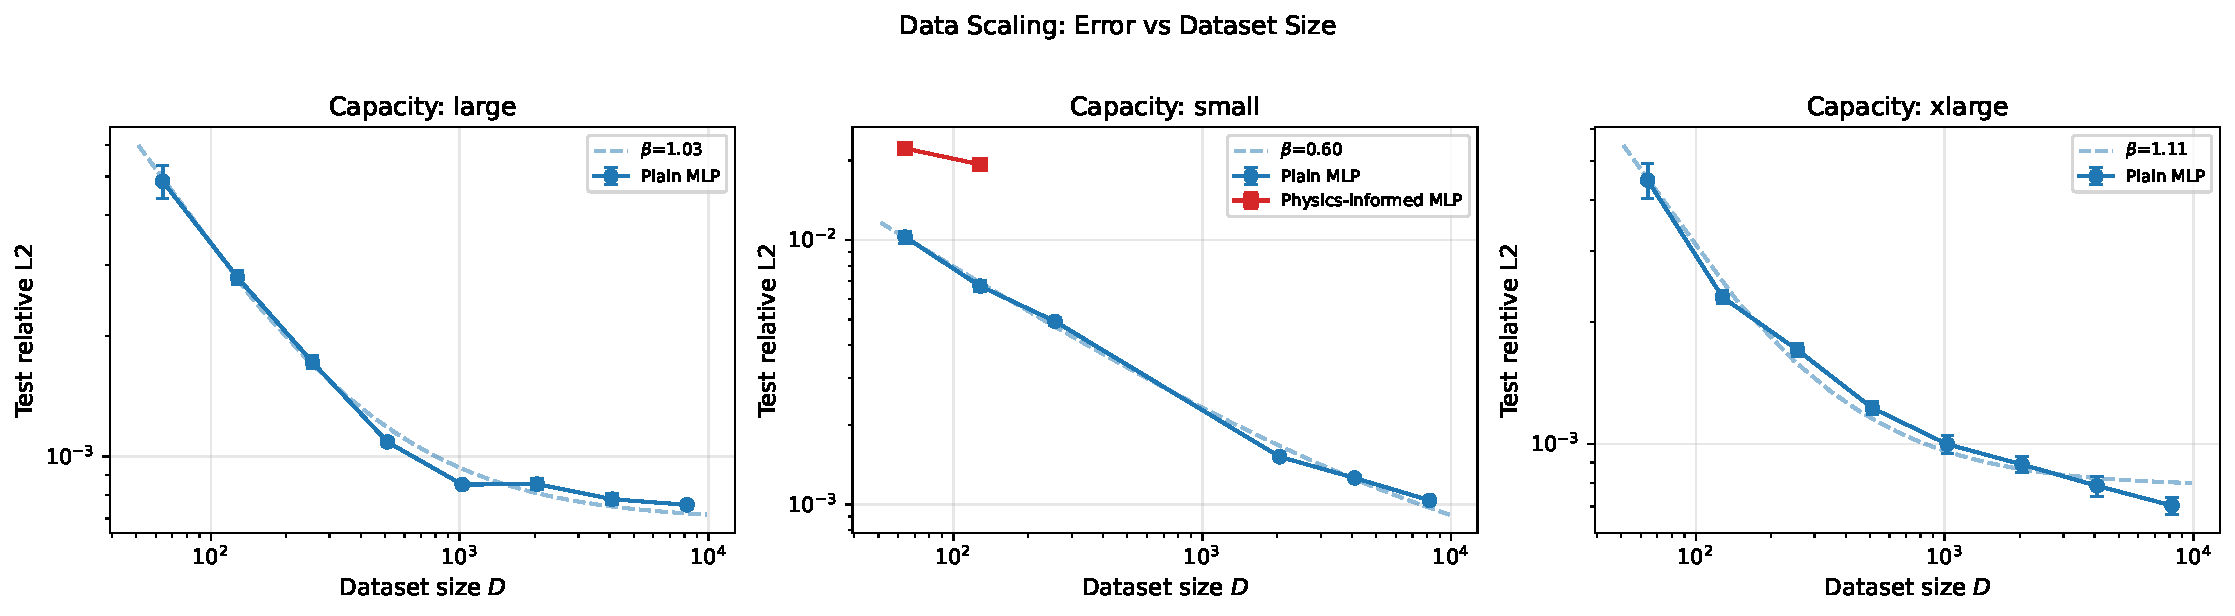
\includegraphics[width=\textwidth]{fig_data_scaling.pdf}
    \caption{Data scaling for all three scaling-law models.
    Left to right: small, medium, and large capacity.
    The plain MLP (blue circles) exhibits clean power-law decay with exponent $\hat{\beta} \approx 0.85$.
    The midpoint-residual PIML (red squares) saturates at $E \approx 0.014$--$0.016$.
    The composite midpoint PIML (green diamonds) tracks below the midpoint and above the plain baseline, with steeper scaling.}
    \label{fig:data-scaling}
\end{figure}

\subsection{ODE-residual prior: biased scaling}
\label{sec:results-midpoint}

\Cref{fig:capacity-scaling} shows the complementary view: test error versus model capacity at fixed dataset sizes.
The plain MLP error decreases steadily with $N$, while the midpoint PIML flattens, confirming that additional capacity cannot overcome the biased prior.

\begin{figure}[H]
    \centering
    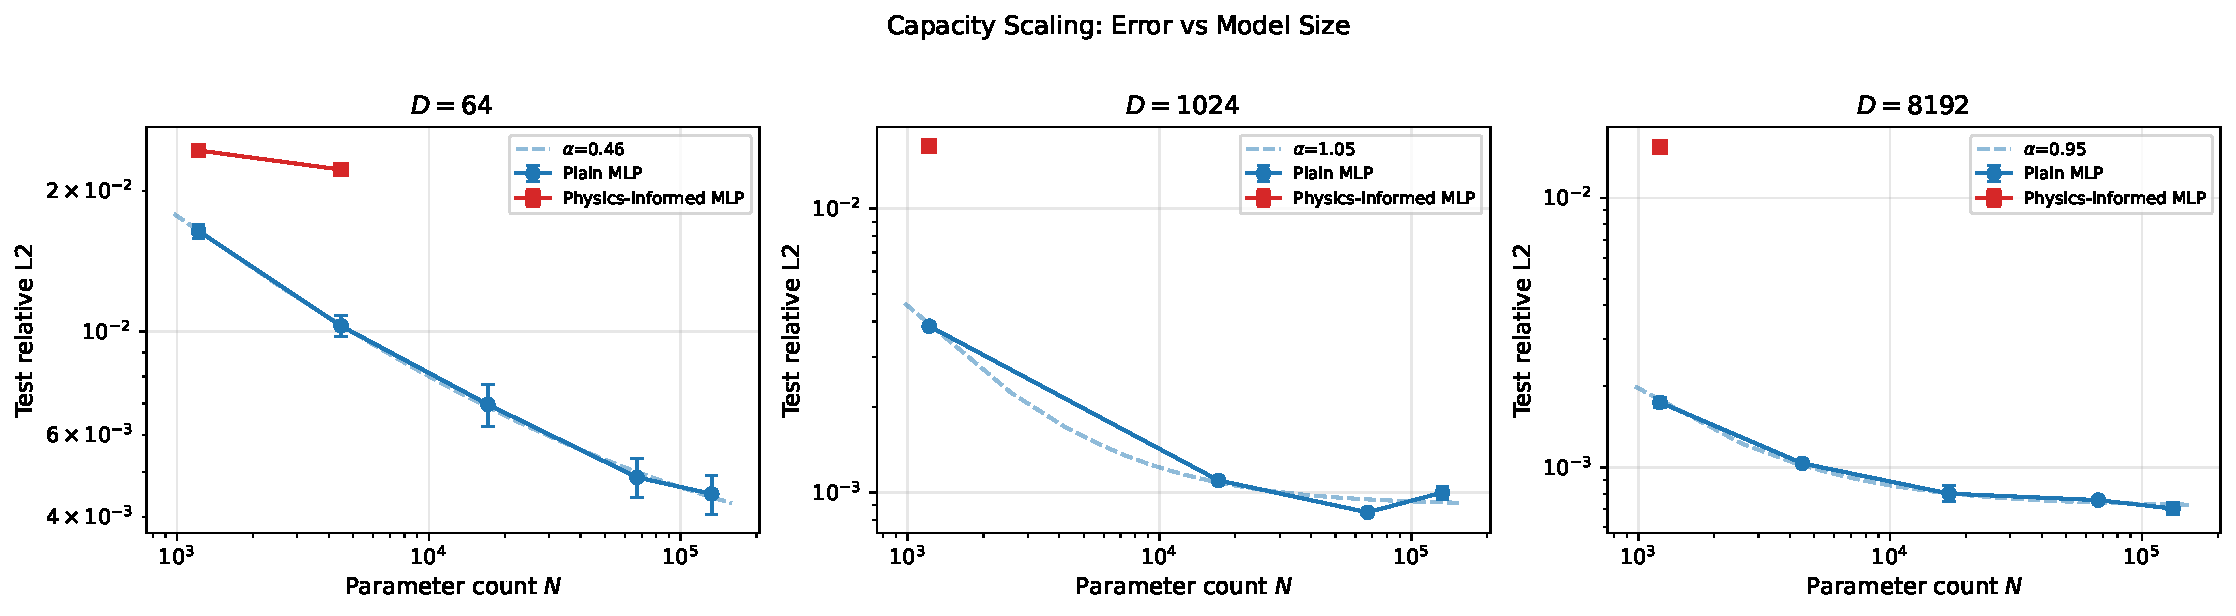
\includegraphics[width=\textwidth]{fig_capacity_scaling.pdf}
    \caption{Capacity scaling: test error versus parameter count $N$ at representative dataset sizes.
    The plain MLP (blue) follows a power law with $\hat{\alpha} \approx 0.93$.
    The midpoint PIML (red) shows minimal improvement beyond the physics-loss plateau.
    The composite PIML (green) exhibits steep capacity scaling, approaching the plain baseline at large $N$.}
    \label{fig:capacity-scaling}
\end{figure}

The midpoint-residual PIML model (with $\lambda_{\mathrm{phys}} = 0.1$) shows qualitatively different scaling behavior.
Test errors plateau at approximately $E \approx 0.014$--$0.016$ across all $(N,D)$ configurations, with weak dependence on either axis:

\begin{center}
\small
\begin{tabular}{lrrrr}
\toprule
& $D = 64$ & $D = 512$ & $D = 2048$ & $D = 8192$ \\
\midrule
Tiny    & $0.0244 \pm 0.0006$ & $0.0176 \pm 0.0002$ & $0.0162 \pm 0.0002$ & $0.0155 \pm 0.0002$ \\
Small   & $0.0222 \pm 0.0006$ & $0.0170 \pm 0.0002$ & $0.0162 \pm 0.0001$ & $0.0155 \pm 0.0002$ \\
Medium  & $0.0202 \pm 0.0008$ & $0.0163 \pm 0.0001$ & $0.0157 \pm 0.0003$ & $0.0148 \pm 0.0003$ \\
Large   & $0.0198 \pm 0.0007$ & $0.0159 \pm 0.0001$ & $0.0150 \pm 0.0005$ & $0.0143 \pm 0.0002$ \\
XLarge  & $0.0192 \pm 0.0007$ & $0.0154 \pm 0.0002$ & $0.0139 \pm 0.0004$ & $0.0141 \pm 0.0002$ \\
\bottomrule
\end{tabular}
\end{center}

The combined scaling fit yields:
\[
\hat{E}_\infty \approx 0.011,\quad \hat{\alpha} \approx 0.16,\quad \hat{\beta} \approx 0.53.
\]
The high error floor (14$\times$ the plain model's best error) and shallow exponents indicate that the prior dominates the optimization, preventing the model from exploiting additional data or capacity.

\begin{figure}[H]
    \centering
    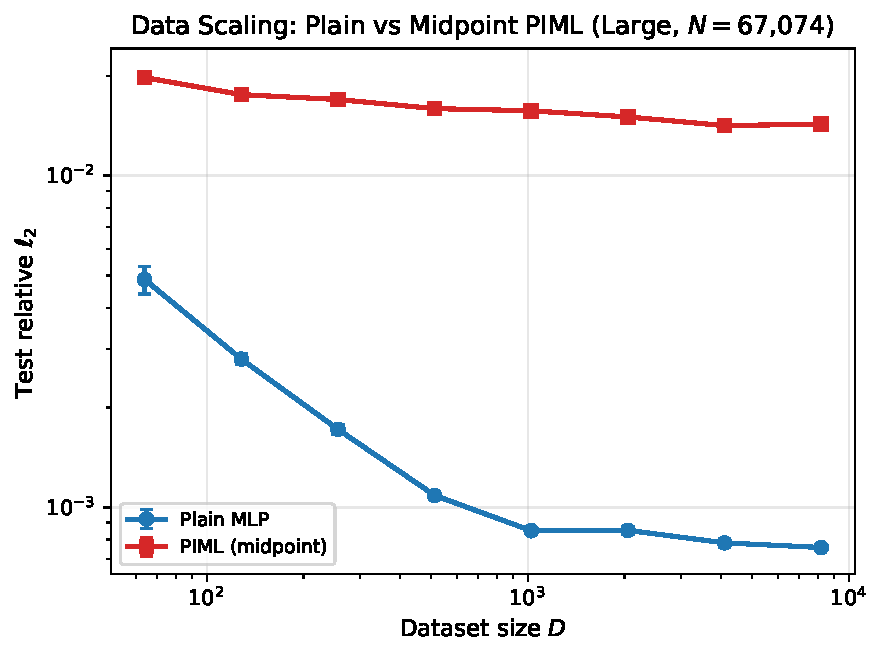
\includegraphics[width=0.7\textwidth]{fig_comparative_data_scaling.pdf}
    \caption{Comparative data scaling at large capacity ($N = 67{,}074$).
    The plain MLP (blue) continues to improve with data.
    The midpoint PIML (red) saturates at $E \approx 0.014$, limited by the biased physics-loss floor.
    The composite PIML (green) tracks $\sim\!1.5\times$ above the plain baseline but declines steadily, reflecting recovered data scaling with a small residual floor.}
    \label{fig:midpoint-vs-plain}
\end{figure}

\paragraph{Interpretation.}
The midpoint-rule residual is a first-order quadrature approximation.
At the tested horizon $T = 1.0$, even ground-truth flow-map targets incur a mean relative residual of approximately 15\% under this approximation.
The physics loss therefore has an irreducible floor of $\mathcal{L}_{\mathrm{mid}}^* \approx 0.15$, which is $\sim\!50{,}000\times$ larger than the achievable data loss ($\sim\!3 \times 10^{-6}$).
As training progresses and data loss decreases, the physics gradient dominates, and the optimizer converges to a plateau determined by the biased prior rather than the data.

\subsection{Conservation-law prior: bimodal optimization failure}
\label{sec:results-conservation}

The conservation-law prior, despite having zero irreducible error on ground-truth targets ($\mathcal{L}_{\mathrm{cons}}^* \approx 10^{-14}$), exhibits a qualitatively different failure mode from the midpoint prior.
Rather than a deterministic error floor, the conservation prior introduces a \emph{bimodal optimization failure}: depending on the random seed, training either converges to the correct basin (matching the plain baseline) or traps in a bad local minimum at test error $\approx 0.09$.

A $\lambda$ sweep across 7 values ($\lambda \in \{0, 10^{-4}, 10^{-3}, 10^{-2}, 10^{-1}, 1, 10\}$) at two capacities and three dataset sizes (126 runs total) reveals the pattern:

\begin{center}
\small
\begin{tabular}{lccccccc}
\toprule
& \multicolumn{7}{c}{$\lambda_{\mathrm{phys}}$} \\
\cmidrule(lr){2-8}
Config & $0$ & $10^{-4}$ & $10^{-3}$ & $10^{-2}$ & $10^{-1}$ & $1$ & $10$ \\
\midrule
Small, $D\!=\!128$  & 0.0061 & 0.0071 & 0.0070 & 0.0068 & 0.0076 & 0.0086 & 0.0156 \\
Small, $D\!=\!1024$ & 0.0022 & 0.0641 & 0.0641 & 0.0021 & 0.0022 & 0.0024 & 0.0038 \\
Small, $D\!=\!4096$ & 0.0013 & 0.0977 & 0.0977 & 0.0468 & 0.0481 & 0.0013 & 0.1153 \\
\midrule
Large, $D\!=\!128$  & 0.0028 & 0.0885 & 0.0885 & 0.0583 & 0.0288 & 0.0030 & 0.2778 \\
Large, $D\!=\!1024$ & 0.0008 & 0.0869 & 0.0869 & 0.0870 & 0.0615 & 0.1141 & 0.2652 \\
Large, $D\!=\!4096$ & 0.0008 & 0.0906 & 0.0906 & 0.0905 & 0.0336 & 0.0511 & 0.1971 \\
\bottomrule
\end{tabular}
\end{center}

\paragraph{Key observations.}
\begin{itemize}[leftmargin=*]
    \item The large model ($N = 67{,}074$) traps at $\approx 0.09$ across nearly all $\lambda > 0$ and $D$ values.
    When it escapes (e.g., $\lambda = 1$, $D = 128$), performance matches the plain baseline.
    \item The small model ($N = 4{,}482$) is less susceptible: it matches or nearly matches the baseline at $\lambda \le 1$ for most dataset sizes, but still traps occasionally at larger $D$.
    \item No value of $\lambda$ consistently improves over the plain baseline.
    \item The pattern is non-monotonic in $\lambda$: trapping depends on the interaction between prior strength, model capacity, and random seed --- unlike the midpoint prior's smooth dose--response curve.
\end{itemize}

\paragraph{Individual seed analysis.}
Examining per-seed results at $\lambda = 0.1$ (large model) reveals the bimodal structure:

\begin{center}
\small
\begin{tabular}{lcccc}
\toprule
$D$ & Seed 101 & Seed 202 & Seed 303 & Trap rate \\
\midrule
128  & 0.003 \checkmark & 0.081 $\times$ & 0.003 \checkmark & 1/3 \\
1024 & 0.088 $\times$ & 0.001 \checkmark & 0.095 $\times$ & 2/3 \\
4096 & 0.099 $\times$ & 0.001 \checkmark & 0.001 \checkmark & 1/3 \\
\bottomrule
\end{tabular}
\end{center}

The trap error ($\approx 0.09$) is a genuine bad local minimum, not a failure to train: an untrained large model gives test error $\approx 0.32$.

\paragraph{Interpretation.}
The conservation constraint $H(\hat{\bm{x}}_T) = H(\bm{x}_0)$ restricts predictions to a 1-dimensional level curve of $H$.
While this manifold contains the correct target, the conservation loss gradient is degenerate along the manifold direction (zero component tangent to the level curve).
This creates ridge-like structures in the combined loss landscape.
Larger models, with their higher-dimensional parameter space, appear more susceptible to these spurious attractors.

\subsection{Composite midpoint prior: recovered scaling}
\label{sec:results-composite}

The composite two-step midpoint prior (\cref{sec:composite-prior}) produces scaling behavior qualitatively different from both the single-step midpoint and the conservation prior.
Representative test errors at large capacity ($N = 67{,}074$):

\begin{center}
\small
\begin{tabular}{lrrrr}
\toprule
& $D = 64$ & $D = 512$ & $D = 2048$ & $D = 8192$ \\
\midrule
Plain       & $0.0049 \pm 0.0005$ & $0.0011 \pm 0.0000$ & $0.0009 \pm 0.0000$ & $0.0008 \pm 0.0000$ \\
Midpoint    & $0.0198 \pm 0.0007$ & $0.0159 \pm 0.0001$ & $0.0150 \pm 0.0005$ & $0.0143 \pm 0.0002$ \\
Composite   & $0.0053 \pm 0.0005$ & $0.0018 \pm 0.0001$ & $0.0013 \pm 0.0001$ & $0.0012 \pm 0.0000$ \\
\bottomrule
\end{tabular}
\end{center}

The composite prior is $3$--$18\times$ better than the single-step midpoint across all configurations, but remains $\sim\!1.1$--$1.6\times$ worse than the plain baseline.
The key insight emerges from the scaling fits rather than the absolute error levels:
\[
\hat{E}_\infty \approx 0.001,\quad \hat{\alpha} \approx 2.0\;[0.26,\, 2.76],\quad \hat{\beta} \approx 1.0\;[0.64,\, 1.63].
\]
The composite prior recovers---and even steepens---the scaling exponents relative to the plain baseline ($\hat{\alpha} \approx 0.93$, $\hat{\beta} \approx 0.87$), while maintaining a near-zero error floor.
The steeper exponents indicate that the composite model benefits \emph{more} from additional capacity and data than the plain model, consistent with the physics loss providing a useful (though imperfect) regularizer once the discretization bias is sufficiently reduced.

The $\sim\!24\times$ reduction in ground-truth physics-loss residual (from $\mathcal{L}_{\mathrm{mid}}^* \approx 0.151$ to $\mathcal{L}_{\mathrm{comp}}^* \approx 0.006$) shifts the model from the approximation-limited regime---where the biased prior dominates---to a regime where both the data and physics gradients provide useful signal.
The remaining $E_\infty \approx 0.001$ floor reflects the residual (but much smaller) discretization bias of the two-step scheme.

\paragraph{Comparison across capacities.}
At medium capacity ($N = 17{,}154$), the composite model achieves $E = 0.0076$ at $D = 64$ and $E = 0.0012$ at $D = 8192$---close to the plain baseline.
At xlarge capacity ($N = 132{,}866$), the composite achieves $E = 0.0049$ at $D = 64$ and $E = 0.0011$ at $D = 8192$, with the gap to plain narrowing as capacity grows.

\subsection{Comparative scaling-law fits}

\Cref{fig:error-heatmap} visualizes the full error surface $E(N,D)$ for all three scaling-law models, and \Cref{fig:exponent-comparison} compares the fitted scaling exponents with bootstrap confidence intervals.

\begin{figure}[H]
    \centering
    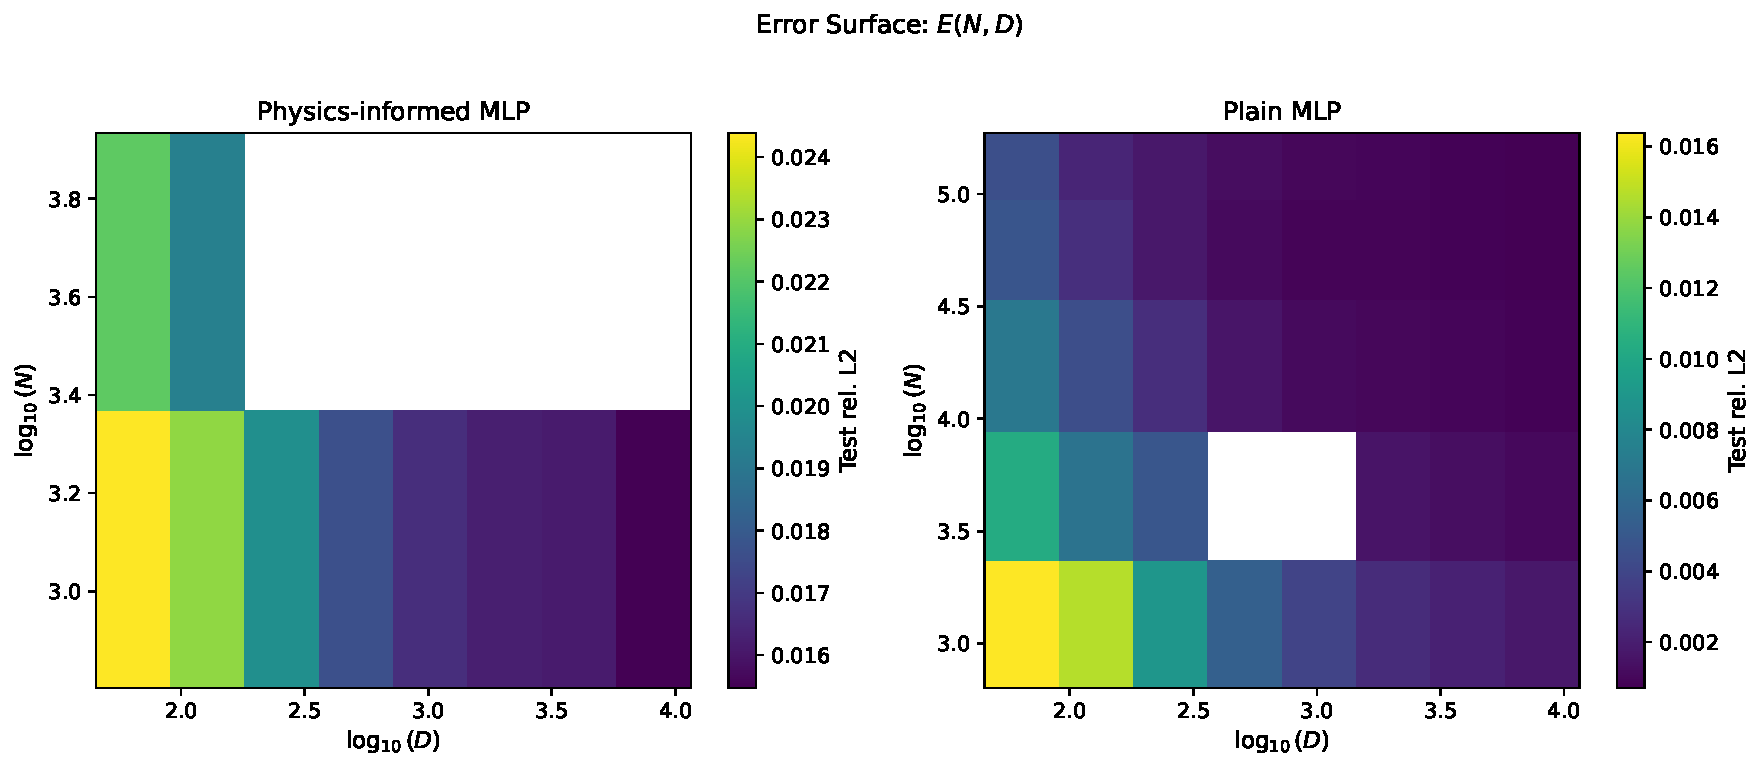
\includegraphics[width=\textwidth]{fig_error_heatmap.pdf}
    \caption{Error surface $E(N,D)$ for the plain MLP (left), midpoint PIML (center), and composite PIML (right).
    The plain model shows a smooth gradient from high error (low $N$, low $D$) to low error (high $N$, high $D$).
    The midpoint PIML is dominated by a uniform plateau near $E \approx 0.015$.
    The composite PIML recovers a smooth gradient similar to plain, shifted slightly upward by its residual floor.}
    \label{fig:error-heatmap}
\end{figure}

\begin{figure}[H]
    \centering
    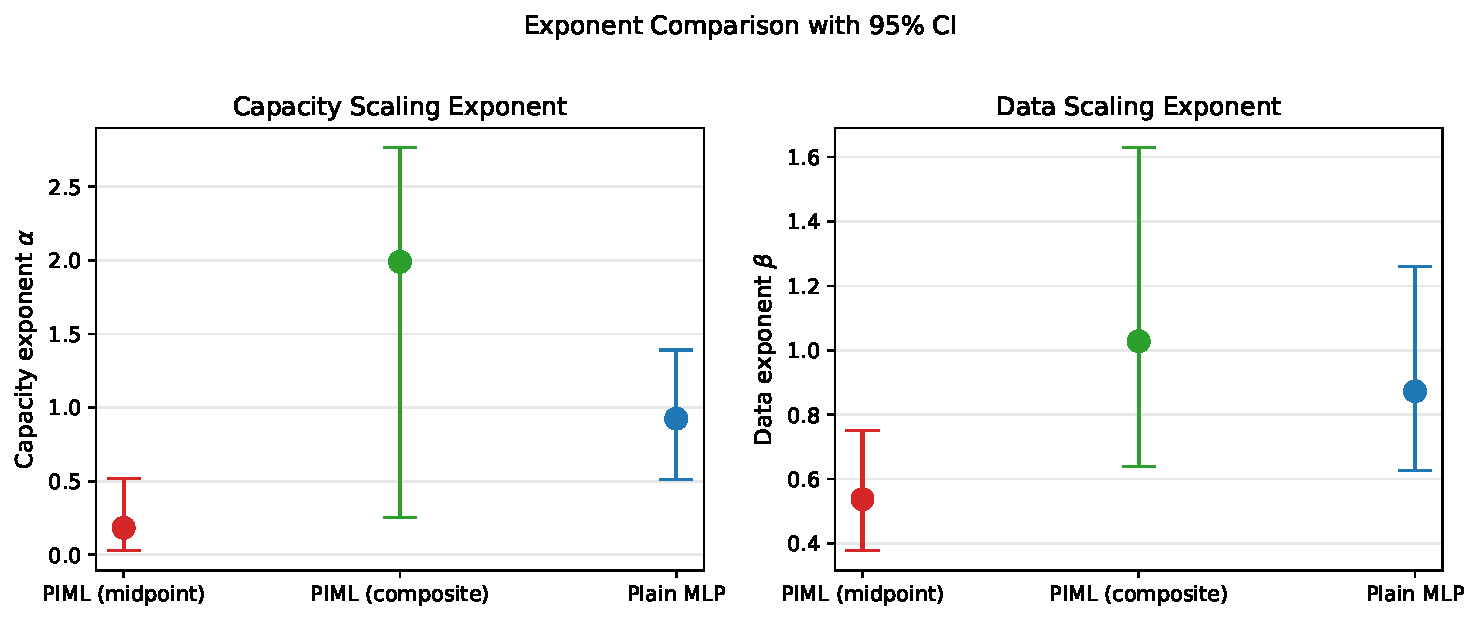
\includegraphics[width=0.8\textwidth]{fig_exponent_comparison.pdf}
    \caption{Fitted scaling exponents with 95\% bootstrap confidence intervals from the joint $E(N,D)$ surface fit.
    Left: capacity exponent $\alpha$.
    Right: data exponent $\beta$.
    The midpoint PIML exponents are substantially compressed, the composite PIML exponents are steeper than plain, and the wide CIs on the composite reflect fewer data points at small capacities.}
    \label{fig:exponent-comparison}
\end{figure}

\begin{table}[H]
    \centering
    \caption{Fitted scaling parameters and failure modes across the four models.
    95\% bootstrap confidence intervals are shown in brackets.}
    \label{tab:scaling-params}
    \begin{tabular}{lcccc}
        \toprule
        Model & $\hat{E}_\infty$ & $\hat{\alpha}$ & $\hat{\beta}$ & Scaling signature \\
        \midrule
        Plain MLP           & $\approx 0$  & 0.93\;[0.51, 1.39] & 0.87\;[0.63, 1.26] & Clean power-law \\
        PIML (midpoint)     & $\approx 0.011$ & 0.18\;[0.03, 0.52] & 0.54\;[0.38, 0.75] & Floor-raising (biased) \\
        PIML (composite)    & $\approx 0.001$ & 2.0\;\;[0.26, 2.76] & 1.0\;\;[0.64, 1.63] & Exponent-steepening \\
        PIML (conservation) & \multicolumn{3}{c}{N/A (bimodal failure)} & Surface-corrupting \\
        \bottomrule
    \end{tabular}
\end{table}

\subsection{Training stability}

All 1{,}080 scaling-law runs (360 each for plain, midpoint, and composite) completed without divergence or NaN.
The midpoint PIML model early-stops substantially earlier: best-epoch values are typically 50--100 versus 300--400 for the plain model, consistent with the optimizer saturating at the physics-loss plateau.
The composite model trains for durations comparable to the plain model, reflecting the continued utility of both data and physics gradients.

The conservation-law prior introduces a distinct stability concern: not divergence, but bimodal convergence.
Approximately 40--70\% of large-model seeds trap in a bad local minimum at test error $\approx 0.09$, while the remainder converge normally.
The small model shows lower trap rates but is not immune.
This stochastic failure mode is qualitatively different from the midpoint prior's deterministic degradation.

\begin{figure}[H]
    \centering
    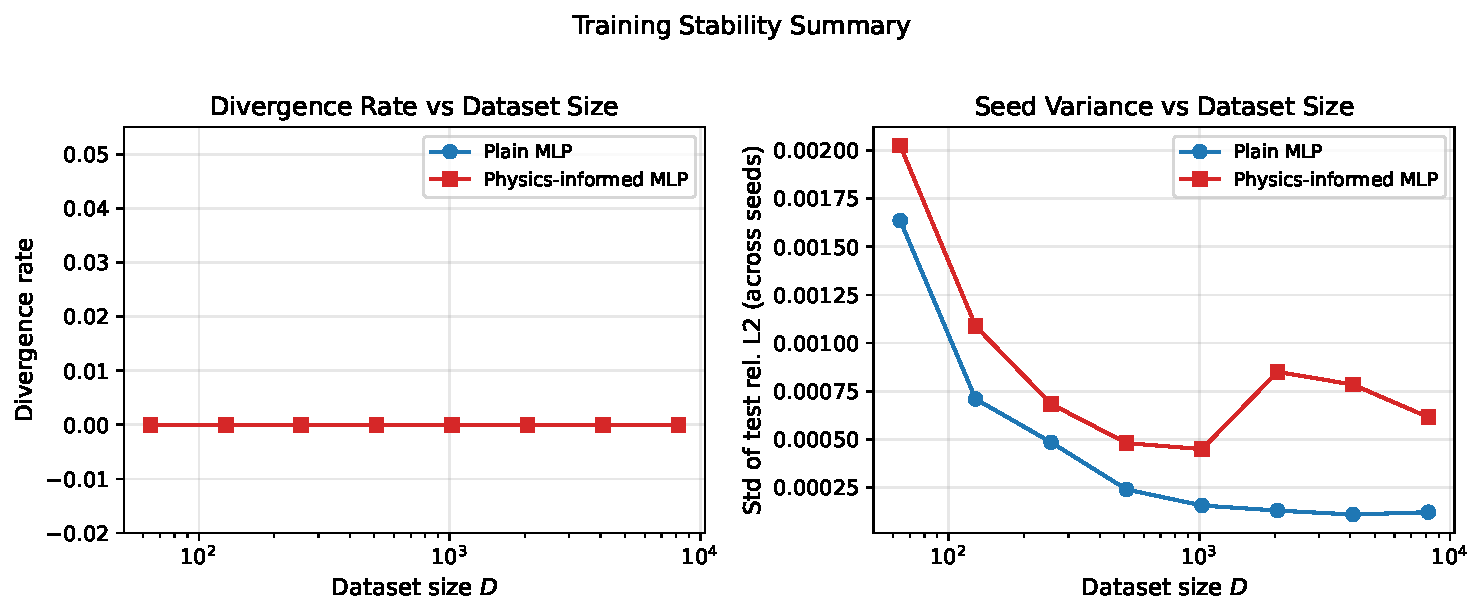
\includegraphics[width=\textwidth]{fig_stability_summary.pdf}
    \caption{Training stability summary.
    Left: divergence rate versus dataset size (zero for all three scaling-law models across all configurations).
    Right: seed-to-seed variance of test error.
    The midpoint PIML exhibits low variance (converging consistently to the physics-loss plateau), while the plain MLP and composite PIML show higher variance at small $D$.}
    \label{fig:stability}
\end{figure}

\subsection{Sensitivity to regularization strength}
\label{sec:results-lambda}

We performed a dedicated $\lambda_{\mathrm{phys}}$ sweep for the midpoint-residual prior across $\lambda \in \{0, 10^{-4}, 10^{-3}, 10^{-2}, 10^{-1}, 1\}$ at two capacities (small, large) and three dataset sizes (128, 1024, 4096), with 9 replicates per configuration (324 runs total).

\begin{table}[H]
    \centering
    \caption{Midpoint-prior $\lambda_{\mathrm{phys}}$ sweep: test relative $\ell_2$ error (mean over 9 replicates).}
    \label{tab:lambda-midpoint}
    \small
    \begin{tabular}{lcccccc}
        \toprule
        & \multicolumn{6}{c}{$\lambda_{\mathrm{phys}}$} \\
        \cmidrule(lr){2-7}
        Config & $0$ & $10^{-4}$ & $10^{-3}$ & $10^{-2}$ & $10^{-1}$ & $1$ \\
        \midrule
        Small, $D\!=\!128$  & 0.0067 & 0.0070 & 0.0068 & 0.0076 & 0.0194 & 0.0748 \\
        Small, $D\!=\!1024$ & 0.0021 & 0.0021 & 0.0021 & 0.0028 & 0.0165 & 0.0711 \\
        Small, $D\!=\!4096$ & 0.0013 & 0.0012 & 0.0012 & 0.0020 & 0.0158 & 0.0706 \\
        \midrule
        Large, $D\!=\!128$  & 0.0028 & 0.0027 & 0.0028 & 0.0035 & 0.0176 & 0.0598 \\
        Large, $D\!=\!1024$ & 0.0009 & 0.0008 & 0.0009 & 0.0019 & 0.0157 & 0.0630 \\
        Large, $D\!=\!4096$ & 0.0008 & 0.0008 & 0.0008 & 0.0015 & 0.0142 & 0.0687 \\
        \bottomrule
    \end{tabular}
\end{table}

Key observations:
\begin{itemize}[leftmargin=*]
    \item $\lambda \le 10^{-3}$: indistinguishable from the plain baseline.
    \item $\lambda = 10^{-2}$: onset of degradation ($1.5$--$2.2\times$ worse).
    \item $\lambda = 10^{-1}$: strong degradation ($8$--$20\times$); error collapses to $\approx 0.015$ regardless of $D$ or $N$.
    \item $\lambda = 1$: severe degradation ($50$--$100\times$).
    \item No value of $\lambda$ improves over the baseline at any configuration.
\end{itemize}
The $\lambda = 0$ path reproduces the plain model bit-for-bit, confirming correct implementation.
The monotonic dose--response pattern rules out isolated hyperparameter failure and is consistent with a biased prior.

The conservation-law $\lambda$ sweep results are presented in \cref{sec:results-conservation} and show a qualitatively different pattern: non-monotonic, seed-dependent trapping rather than smooth degradation.

\begin{figure}[H]
    \centering
    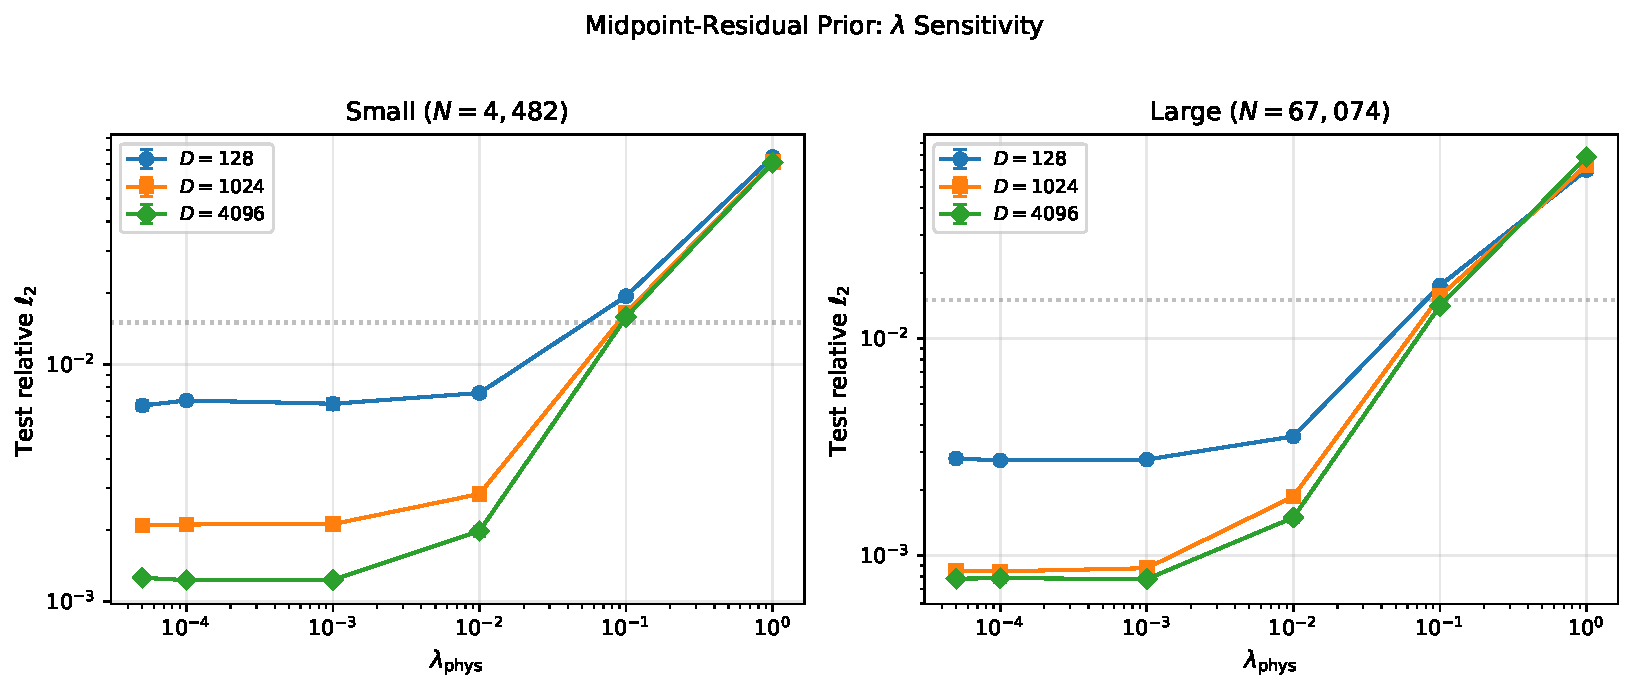
\includegraphics[width=\textwidth]{fig_lambda_midpoint.pdf}
    \caption{Midpoint-residual prior: $\lambda_{\mathrm{phys}}$ sensitivity at small (left) and large (right) capacities.
    The monotonic dose--response pattern is characteristic of a biased prior: increasing $\lambda$ smoothly degrades performance, with no beneficial regime.}
    \label{fig:lambda-midpoint}
\end{figure}

\begin{figure}[H]
    \centering
    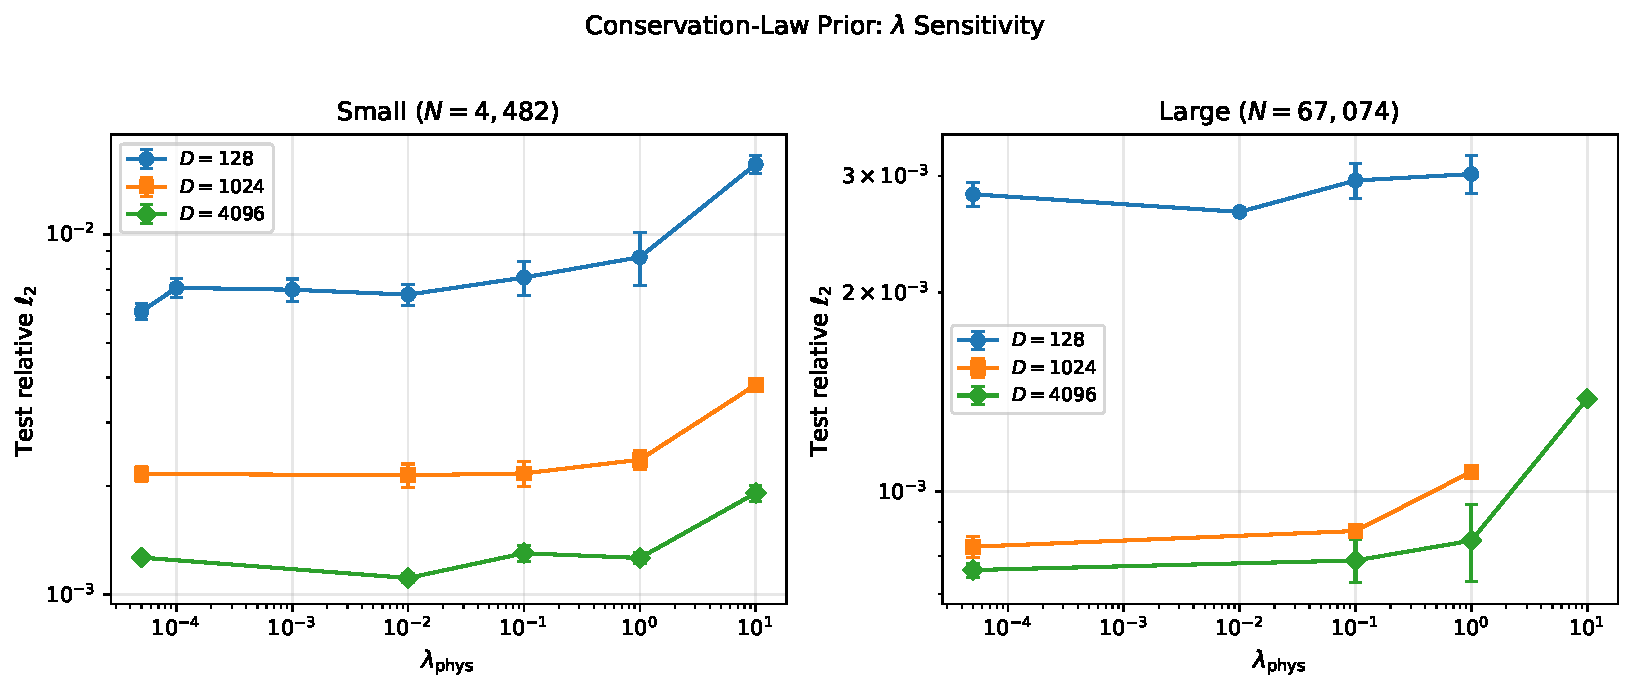
\includegraphics[width=\textwidth]{fig_lambda_conservation.pdf}
    \caption{Conservation-law prior: $\lambda_{\mathrm{phys}}$ sensitivity at small (left) and large (right) capacities.
    Unlike the midpoint prior's smooth degradation, the conservation prior shows non-monotonic behavior with seed-dependent trapping, particularly for the large model at intermediate $\lambda$ values.}
    \label{fig:lambda-conservation}
\end{figure}

%% ================================================================
%%  DISCUSSION
%% ================================================================
\section{Discussion}

\subsection{Scaling signatures as prior diagnostics}

The central finding is that the three physics priors produce three qualitatively distinct scaling signatures (\cref{tab:scaling-params}), which we organize as a diagnostic taxonomy:

\begin{enumerate}[leftmargin=*]
    \item \textbf{Floor-raising (biased proxy).}
    The single-step midpoint prior has irreducible discretization error ($\sim\!15\%$ relative residual on ground truth).
    This elevates $\hat{E}_\infty$ by an order of magnitude and compresses both scaling exponents ($\hat{\alpha}: 0.93 \to 0.18$, $\hat{\beta}: 0.87 \to 0.54$).
    The model becomes insensitive to additional data or capacity.

    \item \textbf{Exponent-steepening (reduced-bias proxy).}
    The composite two-step midpoint prior reduces the ground-truth residual by $\sim\!24\times$.
    This recovers---and steepens---the scaling exponents ($\hat{\alpha} \approx 2.0$, $\hat{\beta} \approx 1.0$) while maintaining a near-zero floor ($\hat{E}_\infty \approx 0.001$).
    The model benefits \emph{more} from additional capacity and data than the plain baseline.

    \item \textbf{Surface-corrupting (exact but informationally weak).}
    The conservation-law prior has zero bias but constrains only a single scalar on a 2-dimensional output.
    Rather than improving scaling, it introduces bimodal optimization failure that worsens with model capacity, precluding power-law fitting.
\end{enumerate}

These three signatures are \emph{not} visible in point-wise comparisons.
At any single $(N,D)$ configuration, both ODE-residual priors underperform the plain baseline in absolute terms; only the scaling exponents and error floors reveal that the single-step prior destroys scaling behavior while the composite prior enhances it.

\subsection{Why the midpoint prior raises the floor}

The midpoint-rule residual approximates $\int_0^T F(\bm{x}(t))\,dt$ with a single evaluation at the midpoint $(\bm{x}_0 + \bm{x}_T)/2$.
At $T = 1.0$, the Lotka--Volterra trajectory curvature makes this approximation poor: ground-truth targets incur $\sim\!15\%$ relative residual.
As the data loss decreases during training, the physics gradient grows relative to the data gradient:
\[
\frac{\lambda \cdot \nabla \mathcal{L}_{\mathrm{mid}}}{\nabla \mathcal{L}_{\mathrm{data}}} \sim \frac{\lambda \cdot O(1)}{O(\mathcal{L}_{\mathrm{data}})},
\]
eventually dominating the optimization.
This mechanism produces the monotonic dose--response degradation in the $\lambda$ sweep (\cref{fig:lambda-midpoint}) and explains both the observed error plateau and the premature early stopping.

\subsection{Why the composite prior recovers scaling}

Halving the step size from $T$ to $T/2$ in the composite scheme reduces the ground-truth physics loss by $\sim\!24\times$ (from $0.151$ to $0.006$; \cref{app:lambda-diagnostic}).
This shifts the model from the approximation-limited regime---where the biased prior floor dominates---into a regime where both data and physics gradients provide useful signal throughout training.

The steeper exponents ($\hat{\alpha} \approx 2.0$ vs.\ $0.93$) suggest that the physics regularization acts as an implicit constraint that accelerates convergence along the capacity and data axes, analogous to how well-matched regularizers improve sample complexity in classical learning theory.
The remaining error floor ($\hat{E}_\infty \approx 0.001$) reflects the residual discretization bias of the two-step scheme and could, in principle, be further reduced with higher-order or multi-step methods.

This result has a practical implication: for ODE-residual priors, the \emph{accuracy of the numerical discretization} determines whether the prior helps or hurts in the scaling limit.
A practitioner can diagnose this by computing the ground-truth residual magnitude---a simple, model-free check that predicts the scaling behavior before any training runs.

\subsection{Why the conservation prior corrupts the surface}

The conservation constraint $H(\hat{\bm{x}}_T) = H(\bm{x}_0)$ is exact yet informationally weak: it constrains a single scalar invariant on a 2-dimensional output.
The level set $\{(u,v) : H(u,v) = c\}$ is a closed curve containing the correct target, but the conservation loss gradient vanishes along the tangent to this curve.
The combined loss landscape acquires ridge-like structures whose severity increases with model capacity: larger models have more degrees of freedom that can align with the degenerate manifold direction.

This pathology is distinct from the training failures reported for PINNs~\cite{wang2022ntk}, which arise from spectral bias and ill-conditioned neural tangent kernels.
The conservation failure is geometric rather than spectral: it stems from the rank deficiency of the constraint Jacobian relative to the output dimension.
Informational sufficiency---whether the physics prior constrains all output degrees of freedom---may be as important as bias-freeness.

\subsection{Implications for prior design}

The three-way taxonomy maps onto a practical design space for physics-informed losses:

\begin{itemize}[leftmargin=*]
    \item \textbf{Soft residual penalties} (e.g., PINN-style collocation losses~\cite{raissi2019pinn,cuomo2022}) impose approximate dynamic constraints.
    Our results show that the \emph{discretization accuracy} determines the scaling outcome: a biased single-step residual raises the error floor, while a reduced-bias composite residual steepens exponents.
    The ground-truth residual magnitude is a simple predictive diagnostic.
    \item \textbf{Exact but partial constraints} (e.g., conservation laws, symmetry penalties) are bias-free but may be informationally insufficient, creating degenerate directions in the loss landscape.
    Our conservation-prior results show that such constraints can introduce capacity-dependent optimization failures even when the prior is theoretically ideal.
    \item \textbf{Hard architectural constraints} (e.g., Hamiltonian or symplectic network structures~\cite{willard2022,chen2018node}) embed physics directly into the parameterization, eliminating certain failure modes by construction.
    Whether architectural constraints produce floor-raising, exponent-steepening, or novel scaling signatures is an open empirical question.
    \item \textbf{Operator-learning architectures} (e.g., DeepONet~\cite{lu2019deeponet}, Fourier Neural Operators~\cite{li2020fno}) encode structural assumptions about the solution operator.
    Theoretical work on neural scaling for elliptic PDEs~\cite{lu2021elliptic} suggests fundamentally different scaling exponents; the taxonomy developed here provides a framework for empirical verification.
\end{itemize}

A key open question is whether the three scaling signatures identified here---floor-raising, exponent-steepening, and surface-corrupting---recur across these different prior classes.

\subsection{Connection to scaling-law theory}

Bahri et al.~\cite{bahri2024} explain neural scaling laws through two limiting regimes: a \emph{variance-limited} regime at small data (where error decreases as $D^{-\beta}$) and a \emph{resolution-limited} regime at small model capacity (where error decreases as $N^{-\alpha}$).
In this framework, the plain MLP in our study operates in a regime where both limitations are active and neither dominates, producing clean power-law behavior across the tested $(N,D)$ grid.

The midpoint prior disrupts this picture by introducing a third limitation: an \emph{approximation-limited} regime in which the irreducible bias of the physics loss creates a floor that dominates both the variance and resolution components.
This floor manifests as the large $\hat{E}_\infty$ and compressed exponents in \cref{tab:scaling-params}.
The composite prior demonstrates that reducing this bias can \emph{exit} the approximation-limited regime, recovering (and steepening) the original scaling behavior.
The conservation prior introduces yet another regime: an \emph{optimization-limited} regime where the loss landscape geometry, rather than data or capacity, determines performance.
These additional regimes are absent from the standard deep-learning scaling framework and may require dedicated theoretical treatment for SciML settings.

The observation that scientific learning problems can be simultaneously variance-limited, resolution-limited, approximation-limited, and optimization-limited---depending on the form of the physics prior---motivates extending scaling-law theory to accommodate structured loss functions and constrained architectures.
Recent surveys of scaling behavior across machine learning settings~\cite{wang2024scaling} document similar anomalies in other structured domains, suggesting that regime transitions driven by inductive-bias mismatch may be a general phenomenon.

\subsection{Toward a scaling-law framework for SciML}

This paper is the first case study in a broader research program that aims to adapt empirical scaling laws to scientific machine learning and use them as a method-agnostic diagnostic for physics-informed priors.
The present results establish the experimental methodology on a minimal dynamical system and identify three qualitative scaling signatures.
The research program is organized around four questions that extend beyond the scope of this initial study:

\begin{enumerate}[leftmargin=*, itemsep=0.3em]
    \item \emph{How should scaling laws be reformulated for dynamical systems and PDE flow maps?}
    The standard ansatz (\cref{eq:scaling}) assumes smooth power-law behavior, which the conservation prior violates.
    Extensions may need to incorporate prediction horizon, discretization resolution, and parameter variability as additional scaling axes.
    \item \emph{Can different physics priors be compared quantitatively through their scaling signatures?}
    Our results show that three priors on the same system produce three distinct and interpretable signatures.
    The next step is to test whether these distinctions persist across PINN-style collocation, architectural constraints, and operator-learning approaches~\cite{raissi2019pinn,li2020fno,lu2019deeponet}.
    \item \emph{Do different forms of inductive bias produce characteristic scaling regimes?}
    The approximation-limited, regularization-enhanced, and optimization-limited regimes identified here may have counterparts for other prior types.
    Connecting these empirical regimes to the variance-limited/resolution-limited framework of Bahri et al.~\cite{bahri2024} and the generalization bounds of Lu et al.~\cite{lu2021elliptic} is a central theoretical goal.
    \item \emph{When do scaling behaviors generalize across systems and when do they diverge?}
    The present study uses a single ODE system.
    Subsequent work will extend to 1D PDEs (diffusion, Burgers, wave equations) as standard PINN and operator-learning benchmarks~\cite{raissi2019pinn,li2020fno}, followed by more complex nonlinear regimes including 2D Navier--Stokes and multiscale closure problems~\cite{sanderse2024}.
\end{enumerate}

The staged design---from analytically tractable ODEs to increasingly complex PDE families---is intended to build understanding progressively, identifying which scaling phenomena are universal and which are system-specific.
A final validation phase will apply the framework to real-world datasets from scientific or industrial contexts to assess whether scaling-based insights obtained under controlled conditions transfer to noisy, imperfect data.

\subsection{Why Lotka--Volterra?}

Lotka--Volterra provides a minimal nonlinear dynamical system that is simple enough for exhaustive sweeps yet nontrivial enough to make inductive bias relevant.
It possesses an exact first integral, enabling a controlled comparison between an exact and an approximate prior on the same task.
The system also generates closed orbits with significant curvature at $T=1.0$, which stresses the midpoint approximation and makes the conservation prior geometrically nontrivial.
Conclusions should not be overgeneralized to PDE learning, chaotic systems, or more complex physics-informed architectures; the purpose of this study is methodological calibration, not broad empirical generalization.

%% ================================================================
%%  LIMITATIONS
%% ================================================================
\section{Limitations}

\begin{enumerate}[leftmargin=*, itemsep=0.3em]
    \item The study uses a single dynamical system (Lotka--Volterra).
    \item It compares a plain MLP against three soft-constraint regularizers; architectural physics priors are not tested.
    \item It focuses on fixed-horizon prediction ($T = 1.0$) rather than long autoregressive rollout.
    \item It uses noise-free synthetic data.
    \item The scaling-law ansatz \cref{eq:scaling} is a descriptive approximation, not a theoretical prediction.
    \item The composite prior's steeper exponents have wide bootstrap confidence intervals ($\hat{\alpha} \in [0.26, 2.76]$), reflecting limited data at small capacities; higher-resolution sweeps would tighten these estimates.
    \item The conservation prior's bimodal failure might be ameliorated by optimization techniques (warm-starting, gradient clipping, adaptive $\lambda$ scheduling) not tested here.
    \item No prior tested here improves over the plain baseline in absolute test error at any configuration; the composite prior's advantage is visible only in scaling exponents and error floor.
\end{enumerate}

%% ================================================================
%%  CONCLUSION
%% ================================================================
\section{Conclusion}

We introduced empirical scaling laws as a diagnostic framework for evaluating physics priors in scientific machine learning.
On fixed-horizon Lotka--Volterra flow-map prediction, we compared a plain MLP against three physics-regularized variants across model capacity and dataset size, totaling over 1{,}400 training runs.

The three priors produce three qualitatively distinct scaling signatures:
\begin{itemize}[leftmargin=*, itemsep=0.2em]
    \item A \emph{biased} ODE-residual prior raises the error floor and compresses scaling exponents ($\hat{\alpha}: 0.93 \to 0.18$, $\hat{\beta}: 0.87 \to 0.54$).
    \item A \emph{reduced-bias} composite ODE-residual prior recovers and steepens scaling ($\hat{\alpha} \approx 2.0$, $\hat{\beta} \approx 1.0$) with a near-zero floor.
    \item An \emph{exact but informationally weak} conservation prior introduces bimodal optimization failures that worsen with model capacity.
\end{itemize}

The main contribution is methodological: scaling laws serve not only as a compact summary of learning behavior, but as a diagnostic tool that reveals \emph{how} a prior modifies the learning surface.
Two priors that both underperform the baseline in absolute terms produce fundamentally different scaling signatures---one destructive, one constructive---that are invisible to point-wise comparisons.
The ground-truth residual magnitude of an ODE-residual prior predicts its scaling behavior before any training runs, providing a simple pre-experimental diagnostic.

This perspective---treating scaling behavior itself as the object of study---supports a more principled basis for evaluating physical inductive biases and motivates extending scaling-law methodology to broader classes of physics-informed methods and PDE systems.

\section*{Acknowledgments}

Acknowledgments placeholder.

%% ================================================================
%%  APPENDICES
%% ================================================================
\appendix

\section{Physics-Loss Weight Diagnostic}
\label{app:lambda-diagnostic}

\subsection{Motivation}

A natural concern in any negative result involving a regularized objective is whether the outcome is caused by an implementation bug, an ill-chosen $\lambda_{\mathrm{phys}}$, or a genuine prior--task mismatch.
This appendix documents a systematic diagnostic that distinguishes these cases.

\subsection{Implementation equivalence control}

With $\lambda_{\mathrm{phys}} = 0$, the PIML code path reproduces the plain model bit-for-bit at all tested configurations (\cref{tab:lambda-midpoint}).
This rules out hidden code-path discrepancies.

\subsection{Ground-truth residual}

Evaluating the physics-loss residuals on exact ground-truth targets:

\begin{center}
\begin{tabular}{lcc}
\toprule
Prior & $\mathcal{L}_{\mathrm{phys}}^*$ on GT & Relative to midpoint \\
\midrule
Single-step midpoint & $0.151$ & $1\times$ (baseline) \\
Composite 2-step midpoint & $0.006$ & $\sim\!24\times$ lower \\
Conservation law & $\sim\!10^{-14}$ & exact \\
\bottomrule
\end{tabular}
\end{center}

For the single-step midpoint:
\[
\text{Mean } \|r\|_2 = 0.363, \qquad
\text{Mean relative residual} \approx 15\%.
\]

\subsection{Interpretation}

The midpoint physics loss has an irreducible floor $\sim\!50{,}000\times$ larger than the achievable data loss.
No value of $\lambda$ can fix this: small $\lambda$ makes the prior invisible; large $\lambda$ drives the optimizer toward the biased proxy.
This creates a characteristic dose--response degradation pattern (\cref{tab:lambda-midpoint}) that is a hallmark of floor-raising prior--task mismatch.

The composite two-step midpoint reduces this floor by $\sim\!24\times$, shifting the balance so that the physics gradient provides useful signal rather than harmful bias.
The resulting scaling behavior (\cref{sec:results-composite}) shows recovered and steepened exponents.

The conservation-law prior shows a contrasting pattern.
Because $\mathcal{L}_{\mathrm{cons}}^* \approx 10^{-14}$, there is no irreducible floor.
However, the conservation constraint is informationally weak: it constrains a single scalar invariant $H$ on a 2-dimensional output.
The resulting loss landscape contains spurious local minima along the conserved manifold, producing bimodal convergence rather than smooth degradation.

\section{Conservation-Law Prior: Details}
\label{app:conservation-details}

The Lotka--Volterra first integral is
\[
H(u,v) = \delta u - \gamma \ln u + \beta v - \alpha \ln v.
\]
The conservation loss penalizes $(\Delta H)^2 = (H(\hat{\bm{x}}_T) - H(\bm{x}_0))^2$.
On ground-truth data, $|\Delta H| / |H| \approx 10^{-7}$, confirming the prior is exact to within numerical integration tolerances.

The conservation loss operates in physical (denormalized) space.
Float32 normalization roundtrip introduces $\sim 10^{-7}$ maximum error, which is negligible.
All training data satisfies strict positivity ($u > 0$, $v > 0$), ensuring the logarithmic terms in $H$ are well-defined.
No negative predictions were observed from untrained models within the tested initial-condition domain $[0.5, 2.5]^2$.

The bimodal optimization failure described in \cref{sec:results-conservation} is not caused by numerical issues in the loss computation, but by the geometric structure of the conservation constraint: $H(u,v) = c$ defines a closed curve in $(u,v)$ space, and the conservation gradient is zero along this curve.
This creates a degenerate direction in the combined loss landscape that becomes problematic as model capacity increases.

%% ================================================================
%%  BIBLIOGRAPHY
%% ================================================================
\bibliographystyle{plain}
\begin{thebibliography}{99}

\bibitem{bahri2024}
Y.~Bahri, E.~Dyer, J.~Kaplan, J.~Lee, and U.~Sharma.
\newblock Explaining neural scaling laws.
\newblock \emph{Proceedings of the National Academy of Sciences}, 121(30), 2024.

\bibitem{chen2018node}
R.~T.~Q. Chen, Y.~Rubanova, J.~Bettencourt, and D.~Duvenaud.
\newblock Neural ordinary differential equations.
\newblock In \emph{Advances in Neural Information Processing Systems}, 2018.

\bibitem{cuomo2022}
S.~Cuomo, V.~S. Di~Cola, F.~Giampaolo, G.~Rozza, et al.
\newblock Scientific machine learning through physics-informed neural networks:
  Where we are and what's next.
\newblock \emph{Journal of Scientific Computing}, 92, 2022.

\bibitem{hestness2017}
J.~Hestness, S.~Narang, N.~Ardalani, et al.
\newblock Deep learning scaling is predictable, empirically.
\newblock arXiv:1712.00409, 2017.

\bibitem{henighan2020}
T.~Henighan, J.~Kaplan, M.~Katz, et al.
\newblock Scaling laws for autoregressive generative modeling.
\newblock arXiv:2010.14701, 2020.

\bibitem{kaplan2020}
J.~Kaplan, S.~McCandlish, T.~Henighan, et al.
\newblock Scaling laws for neural language models.
\newblock arXiv:2001.08361, 2020.

\bibitem{karpatne2022}
A.~Karpatne, R.~Kannan, and V.~Kumar.
\newblock \emph{Knowledge Guided Machine Learning: Accelerating Discovery Using Scientific Knowledge and Data}.
\newblock Chapman \& Hall/CRC, 2022.

\bibitem{kashinath2021}
K.~Kashinath, M.~Mustafa, A.~Albert, et al.
\newblock Physics-informed machine learning: Case studies for weather and climate modelling.
\newblock \emph{Philosophical Transactions of the Royal Society A}, 379(2194), 2021.

\bibitem{li2020fno}
Z.~Li, N.~Kovachki, K.~Azizzadenesheli, et al.
\newblock Fourier neural operator for parametric partial differential equations.
\newblock arXiv:2010.08895, 2020.

\bibitem{lu2019deeponet}
L.~Lu, P.~Jin, and G.~E. Karniadakis.
\newblock {DeepONet}: Learning nonlinear operators for identifying differential equations based on the universal approximation theorem of operators.
\newblock arXiv:1910.03193, 2019.

\bibitem{lu2021elliptic}
Y.~Lu, H.~Chen, J.~Lu, L.~Ying, and J.~Blanchet.
\newblock Machine learning for elliptic {PDE}s: Fast rate generalization bound, neural scaling law and minimax optimality.
\newblock arXiv:2110.06897, 2021.

\bibitem{pang2019fpinns}
G.~Pang, L.~Lu, and G.~E. Karniadakis.
\newblock f{PINNs}: Fractional physics-informed neural networks.
\newblock \emph{SIAM Journal on Scientific Computing}, 41(4), 2019.

\bibitem{raissi2019pinn}
M.~Raissi, P.~Perdikaris, and G.~E. Karniadakis.
\newblock Physics-informed neural networks: A deep learning framework for solving forward and inverse problems involving nonlinear partial differential equations.
\newblock \emph{Journal of Computational Physics}, 378:686--707, 2019.

\bibitem{rosenfeld2019}
J.~S. Rosenfeld, A.~Rosenfeld, Y.~Belinkov, and N.~Shavit.
\newblock A constructive prediction of the generalization error across scales.
\newblock arXiv:1909.12673, 2019.

\bibitem{ren2025}
Z.~Ren, S.~Zhou, D.~Liu, and Q.~Liu.
\newblock Physics-informed neural networks: A review of methodological evolution, theoretical foundations, and interdisciplinary frontiers.
\newblock \emph{Applied Sciences}, 15(14), 2025.

\bibitem{sanderse2024}
B.~Sanderse, P.~Stinis, R.~Maulik, and S.~E. Ahmed.
\newblock Scientific machine learning for closure models in multiscale problems: A review.
\newblock arXiv:2403.02913, 2024.

\bibitem{wang2024scaling}
C.~Wang, Y.~Wang, Z.~Li, Q.~Jia, and W.~Liu.
\newblock Scaling laws of data-driven machine learning models: A survey and taxonomy.
\newblock TechRxiv, 2024.

\bibitem{wang2022ntk}
S.~Wang, X.~Yu, and P.~Perdikaris.
\newblock When and why {PINNs} fail to train: A neural tangent kernel perspective.
\newblock \emph{Journal of Computational Physics}, 449, 2022.

\bibitem{willard2022}
J.~Willard, X.~Jia, S.~Xu, M.~Steinbach, and V.~Kumar.
\newblock Integrating scientific knowledge with machine learning for engineering and environmental systems.
\newblock \emph{ACM Computing Surveys}, 54(4), 2022.

\end{thebibliography}

\end{document}
